\chapter{Metodologia}
\label{cap3}

\section{Resumo}

\paragraph{} As seções a seguir trazem detalhes quanto a estrutura técnica do projeto. Portanto, a Figura \ref{fig:100} apresenta uma noção geral de como as estrutras se conectam.

\begin{figure}[h]
    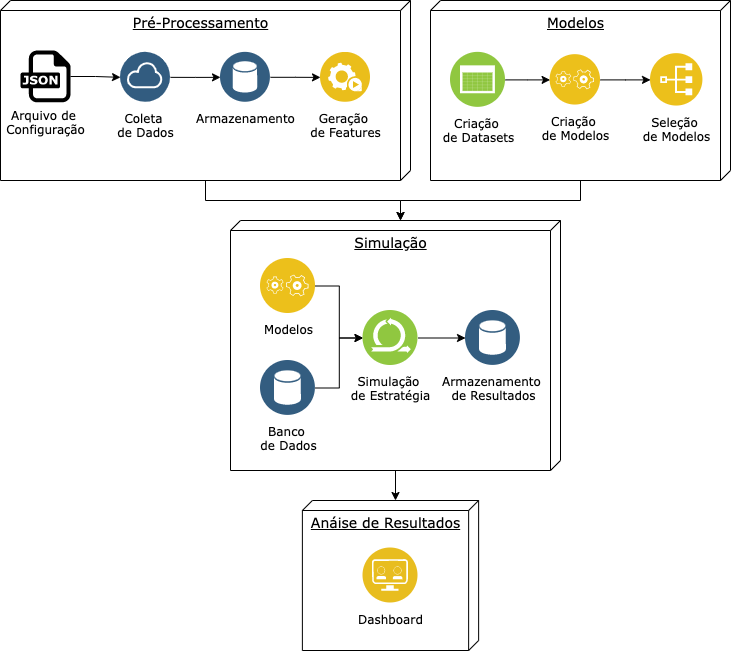
\includegraphics[scale=0.52]{resumo_projeto.png}
    \centering
    \caption{Estrutura do técnica do projeto}
    \label{fig:100}
\end{figure}

\paragraph{} Primeiro, antes da execução do código principal, é necessário garantir que os modelos estão devidamente localizados em pasta apropriada. Para isso, faz-se imprescindível a criação dos \textit{datasets} para cada ação a ser simulada, pois servem de entrada de dados para a criação e seleção dos modelos, etapa esta que deve ser executada logo em sequência. A biblioteca \textit{multiprocessing} foi utilizada para minimizar o tempo total gasto nestas etapas.

\paragraph{} Após a criação dos modelos, tem-se início a etapa de pré-processamento de dados, onde ocorre a leitura e interpretação do arquivo de configuração para se obter o número de estratégias a executar, quais os ativos envolvidos e seus recpectivos intervalos de tempo. Uma vez verificado no banco os dados já existentes, faz-se um \textit{download} apenas dos dados necessários. Se houver alguma atualização de dados, as \textit{features} de uso geral são (re)calculadas e armazenadas no banco a fim de servir de insumo para as estratégias que estarão por vir.

\paragraph{} Completada a etapa de pré-processamento, inicia-se a simulação das estratégias. O arquivo de configuração foi projetado para ser capaz de designar diversas estratégias de parâmetros distintos a uma mesma ordem de execução de programa. Também fez-se uso da biblioteca \textit{multiprocessing} para paralelizar as simulações, cujos resultados e estatísticas são salvas no banco para posterior análise.

\paragraph{} Por fim, é possível visualizar os resultados de forma clara através de uma aplicação secundária responsável por criar um \textit{dashboard} interativo.

\paragraph{} Em relação às tecnologias utilizadas, a aplicação foi desenvolvida em \textit{Python} com o apoio das bibliotecas \textit{yfinance}, \textit{pandas}, \textit{dash} e \textit{multiprocessing}. Foi estruturado um banco de dados \textit{PostgreSQL} para armazenamento dos \textit{candlesticks} obtidos, das \textit{features} geradas e das estratégias simuladas. Também foi incorporado o uso de \textit{Docker} especificamente para a execução de estratégias sem a necessidade de configuração de ambiente.

\section{Pré-Processamento}

\subsection{Arquivo de Configuração}

\paragraph{} O Arquivo de Configuração é um arquivo no formato JSON responsável por configurar detalhadamente cada parâmetro da sequência de estratégias que se deseja executar. Uma ordem de execução do programa pode conter diversas simulações de estratégias, que são configuradas neste Arquivo. A Figura \ref{fig:101} mostra sua estrutura.

\begin{figure}[h]
    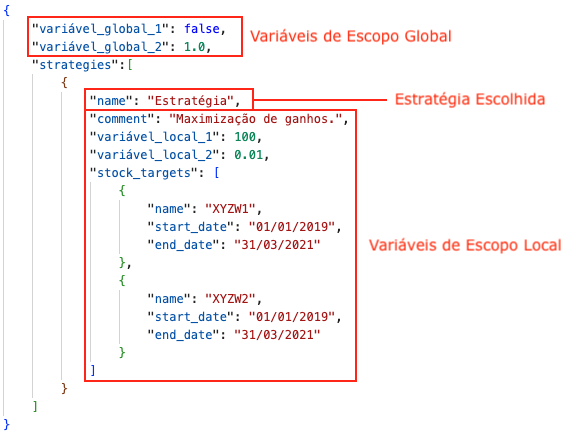
\includegraphics[scale=0.50]{config_file_estrutura.png}
    \centering
    \caption{Estrutura do Arquivo de Configuração}
    \label{fig:101}
\end{figure}

\paragraph{} Nota-se que no topo são listados os parâmetros de uso geral, ou variáveis de escopo global, de cujos valores precedem quaisquer outros listados a seguir, em caso de sobreposição. Em seguida abre-se o vetor de tipos de estratégias, onde o campo \textit{name} representa o nome da classe selecionada, sendo este o elemento que conecta o usuário ao tipo de estratégia desejada. Após a seleção do nome, são configurados os parâmetros internos da estratégia. A Tabela \ref{tab:1} descreve todos os parâmetros disponíveis.

\paragraph{} Para se criar mais de um perfil de simulação, é necessário modificar o Arquivo conforme a Figura \ref{fig:102}. Automaticamente, o código interpreta que existe mais de uma simulação a executar, com todos os parâmetros em comum exceto aqueles em formato de listas. Caso haja mais de um parâmetro no formato de lista, seus comprimentos precisam ser iguais. No caso da Figura \ref{fig:102}, a primeira simulação utilizará os valores (100, 0.01) para o par (variável\_local\_1, variável\_local\_2), a segunda utilizará (200, 0.02) e assim sucessivamente.

\begin{figure}[h]
    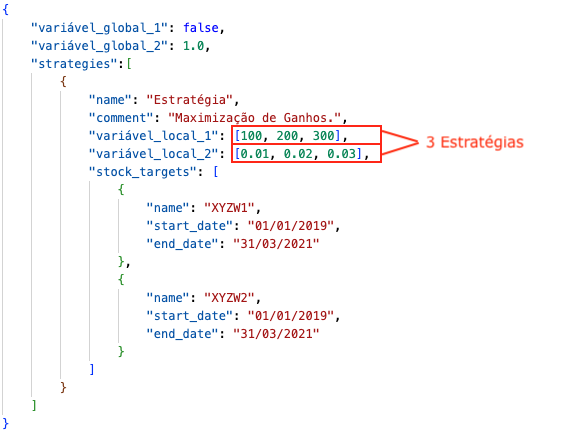
\includegraphics[scale=0.50]{config_file_mult_exec.png}
    \centering
    \caption{Arquivo de Configuração para Execuções Múltiplas}
    \label{fig:102}
\end{figure}

\begin{center}
    {\small
    \begin{longtable}[m]{| m{11em} | m{3em}| m{21em} |}

        \hline
        \multicolumn{3}{|c|}{Lista de Parâmetros} \\
        \hline
        Nome do Parâmetro & Escopo & Descrição \\
        \hline
        \endfirsthead

        \hline
        \multicolumn{3}{|c|}{Continuação da Tabela \ref{tab:1}} \\
        \hline
        Nome do Parâmetro & Escopo & Descrição \\
        \hline
        \endhead

        \hline
        \endfoot

        \hline
        \multicolumn{3}{|c|}{Fim da Tabela \ref{tab:1}} \\
        \hline
        \caption{Lista de parâmetros detalhados.\label{tab:1}}
        \endlastfoot

        \hline
        show\_results & Geral & Exibe \textit{dashboard} da última simulação completada ao final. Tipo: \textit{Boolean}. \textit{Default}: \textit{True}. Listável: Não. \\
        \hline
        min\_risk\_features & Geral & Risco mínimo para o cálculo de \textit{features}. Tipo: \textit{Float}. \textit{Default}: 0,01. Listável: Não. \\
        \hline
        max\_risk\_features & Geral & Risco máximo para o cálculo de \textit{features}. Tipo: \textit{Float}. \textit{Default}: 0,10. Listável: Não. \\
        \hline
        \textbf{name} & Local & \textbf{(OBRIGATÓRIO)} Nome da estratégia a ser executada. Valores válidos: ``ML Derivation". Tipo: \textit{String}. Listável: Não. \\
        \hline
        comment & Local & Comentário. Tipo: \textit{String}. \textit{Default}: \textit{String} vazia. Listável: Não. \\
        \hline
        capital & Local & Capital total da carteira em reais (R\$). Tipo: \textit{Float}. Listável: Sim. \\
        \hline
        risk\_capital\_coefficient & Local & Coeficiente de risco-capital (RCC) geral. Tipo: \textit{Float}. \textit{Default}: 0,001. Listável: Sim. \\
        \hline
        tickers\_bag & Local & Grupo de ativos a escolher dentro de ``stock\_targets". Valores aceitos: ``listed\_first" (ordem de listagem); ``random" (ordem aleatória). \textit{Default}: ``listed\_first". Listável: Sim. \\
        \hline
        tickers\_number & Local & Número de ativos a escolher dentro de ``stock\_targets", de acordo com ``tickers\_bag". Tipo: \textit{Int}. \textit{Default}: 0 (todos). Listável: Sim. \\
        \hline
        min\_order\_volume & Local & Volume mínimo por operação. Tipo: \textit{Int}. \textit{Default}: 1. Listável: Sim. \\
        \hline
        gain\_loss\_ratio & Local & Razão entre ganho e perda. Para uma unidade de risco (delta pencentual entre preço de compra e \textit{stop loss}) são utilizadas N unidades de risco acima no preço preço de compra para definir o preço alvo. Tipo: \textit{Float}. \textit{Default}: 3. Listável: Sim. \\
        \hline
        max\_days\_per\_operation & Local & Número máximo de dias por operação. Inclui o dia de compra. Caso excedido, ocorre venda compulsória pelo preço de fechamento no último dia da contagem. Tipo: \textit{Int}. \textit{Default}: 45. Listável: Não. \\
        \hline
        min\_risk & Local & Risco mínimo por operação. Tipo: \textit{Float}. \textit{Default}: 0,003. Listável: Sim. \\
        \hline
        max\_risk & Local & Risco máximo por operação. Tipo: \textit{Float}. \textit{Default}: 0,10. Listável: Sim. \\
        \hline
        max\_risk & Local & Risco máximo por operação. Tipo: \textit{Float}. \textit{Default}: 0,10. Listável: Sim. \\
        \hline
        enable\_frequency\hspace{2em} \_normalization & Local & Uso de normalização por frequência de operações. Ativos com N vezes mais operações que a média receberão N vezes menos capital. Ver Seção \ref{freq_norm}. Tipo: \textit{Boolean}. \textit{Default}: \textit{False}. Listável: Sim. \\
        \hline
        enable\_profit\hspace{4em} \_compensation & Local & Uso de compensação por lucratividade acumulada. Ver Seção \ref{profit_comp}. Tipo: \textit{Boolean}. \textit{Default}: \textit{False}. Listável: Sim. \\
        \hline
        enable\_crisis\_halt & Local & Bloqueio de novas aquisições em caso de identificação de potenciais crises financeiras (para ativo). Ver Seção \ref{crisis_halt}. Tipo: \textit{Boolean}. \textit{Default}: \textit{False}. Listável: Sim. \\
        \hline
        enable\_downtrend\_halt & Local & Bloqueio de novas aquisições em caso de identificação de tendências de baixo nos preços (para ativo). Ver Seção \ref{downtrend_halt}. Tipo: \textit{Boolean}. \textit{Default}: \textit{False}. Listável: Sim. \\
        \hline
        enable\_dynamic\_rcc & Local & Uso de Coeficiente de Risco-Capital dinâmico (para carteira). Ver Seção \ref{dynamic_rcc}. Tipo: \textit{Boolean}. \textit{Default}: \textit{False}. Listável: Sim. \\
        \hline
        dynamic\_rcc\_reference & Local & Valor de referência de uso de capital médio no controle do RCC dinâmico. Ver Seção \ref{dynamic_rcc}. Tipo: \textit{Float}. \textit{Default}: 0,80. Listável: Sim. \\
        \hline
        dynamic\_rcc\_k & Local & Valor do ganho proporcional K no controle do RCC dinâmico. Ver Seção \ref{dynamic_rcc}. Tipo: \textit{Float}. \textit{Default}: 3. Listável: Sim. \\
        \hline

        purchase\_margin & Local & Margem percentual aplicada ao valor de compra. Ex: Se o alvo de compra estiver configurado para R\$100, uma margem de 1\% permitirá a compra antecipada em R\$99. Tipo: \textit{Float}. \textit{Default}: 0. Listável: Sim. \\
        \hline
        stop\_margin & Local & Margem percentual aplicada ao valor do \textit{stop loss}. Ex: Se o \textit{stop} estiver configurado para R\$100, uma margem de 1\% permitirá a compra antecipada em R\$101. Tipo: \textit{Float}. \textit{Default}: 0. Listável: Sim. \\
        \hline
        partial\_sale & Local & Uso de saídas parciais. Tipo: \textit{Boolean}. \textit{Default}: \textit{False}. Listável: Sim. \\
        \hline
        stop\_type & Local & Tipo de \textit{stop loss} utilizado. Valores aceitos: ``normal"; ``staircase" (para cada patamar de unidade de risco que o preço atinge acima do valor de compra, o \textit{stop} sobe igualmente, até uma unidade de risco abaixo do preço alvo). Ver ``gain\_loss\_ratio". \textit{Default}: ``normal". Listável: Sim. \\
        \hline
        min\_days\_after\_successful \_operation & Local & Mínimo de dias sem novas aquisições após operação de sucesso, para cada ação. Ex: para 1 dia mínimo, se a última venda de sucesso ocorreu durante o dia X, a próxima compra só ocorrerá a partir do dia X+2, inclusive. Tipo: \textit{Int}. \textit{Default}: 0. Listável: Sim. \\
        \hline
        max\_days\_after\_failure \_operation & Local & Mínimo de dias sem novas aquisições após operação de falha, para cada ação. Ex: para 1 dia mínimo, se a última venda de falha ocorreu durante o dia X, a próxima compra só ocorrerá a partir do dia X+2, inclusive. Tipo: \textit{Int}. \textit{Default}: 0. Listável: Sim. \\
        \hline

        \textbf{stock\_targets} & Local & \textbf{(OBRIGATÓRIO)} \textit{Array} de ações a incluir na carteira. Formato indicado pela Figura \ref{fig:101}. Atenção ao parâmetro ``tickers\_bag". \\
        \hline

    \end{longtable}}
\end{center}



\subsection{Coleta de Dados}

\paragraph{} EXCLUIR - yfinance; Problema com proventos; Normalização de proventos do preço das ações.

\paragraph{} A Coleta de Dados ocorre através da biblioteca \textit{open-source} \textit{yfinance} \cite{yfinance}, uma ferramenta de terceiros que transmite dados públicos da plataforma \textit{Yahoo! Finance} \cite{yahoo_finance}, um subsistema da rede \textit{Yahoo!}.

\paragraph{} A escolha desta biblioteca como fonte de dados se deve à sua gratuidade e facilidade de uso, porém após alguns tester e verificações com outras fontes, deve-se ressaltar algumas questões.

\begin{itemize}
    \item Os valores de proventos que a biblioteca disponibiliza não são consistentes, portanto não são utilizados por este projeto. Testes internos confirmaram a presença de diversos valores de dividendos e juros sobre capital próprio corretamente apresentados e ajustados pelos desdobramentos acumulados, porém somados a alguns \textit{outliers} inexistentes na realidade, o suficiente para questionar seu uso em escala (i.e., para vários ativos sem verificação individual).
    \item PROVENTOS EMBUTIDOS NO PREÇO DAS AÇOES?
    \item DIA DE MEIO EXPEDIENTE NO CARNAVAL
    \item VERIFICACAO COM TRADING VIEW
\end{itemize}

\paragraph{} Os dados obtidos são \textit{candlesticks} diários (OHLCV). Com a mesma facilidade, é possível adquirir janelas de tempo semanais, no entanto para evitar potenciais problemas de consistência de dados, as mesmas são calculadas internamente a partir da janela diária via comandos SQL\footnote{\textit{Structured Query Language}: Linguagem usada para administrar bancos de dados relacionais.}.







\subsection{Armazenamento de Dados}
\paragraph{} EXCLUIR - Banco de dados; Criação de Candles semanais.

\subsection{Geração de \textit{Features} de Uso Geral}
\paragraph{} EXCLUIR - Quais features; Cuidados com não-causalidade.


\section{Simulação de Estratégia}

\subsection{Estrutura}
\paragraph{} EXCLUIR - Carteira com N ativos de datas distintas; Regra de 3 para 1 entre stop e alvo; 1 operação por ativo.

\subsection{Premissas}
\paragraph{} EXCLUIR - Compra na abertura do merdado; Sem venda no dia da compra; Prioridades durante venda (stop primeiro).

\subsection{Período Máximo de Dias por Operação}
\paragraph{} EXCLUIR - Motivação da escolha dos 45 dias; Gráfico entre ABEV e MGLU.

\subsection{Gerenciamento de Risco}
\paragraph{} EXCLUIR - Coeficiente de Risco-Capital

\subsection{Risco de Entrada por Operação}
\paragraph{} EXCLUIR - Cálculo do risco mínimo; Cálculo do risco Máximo.

\subsection{Descanso por Tendência de Baixa}
\label{downtrend_halt}
\paragraph{}

\subsection{Descanso por Identificação de Crises}
\label{crisis_halt}
\paragraph{}

\subsection{Lista de Parâmetros de Configuração}
\paragraph{} EXCLUIR - Lista todos e explicar o que fazem.

\subsection{Ensaios Paralelos}
\paragraph{} EXCLUIR - Parâmetros que estão implementados e não trouxeram resultados expressivos.



\section{Otimizações de Gerenciamento de Carteira}

\subsection{Normalização por Frequência de Operações}
\label{freq_norm}
\paragraph{}

\subsection{Compensação por Lucratividade}
\label{profit_comp}
\paragraph{}

\subsection{Controle Proporcional para Uso de Capital}
\label{dynamic_rcc}
\paragraph{}




\section{Criação de Modelos}

\subsection{Resumo}
\paragraph{}

\subsection{\textit{Feature Selection}}
\paragraph{}

\subsection{Geração de \textit{Datasets}}
\paragraph{}

\subsection{\textit{Walk Forward Optimization}}
\paragraph{}

\subsection{Critérios de Escolha}
\paragraph{}


\section{Análise de Resultados}
\paragraph{} EXCLUIR - Dashboard; Baseline